%%%%%%%%%%%%%%%%%%%%%%%%%%%%%%%%%%%%%%%%%%%%%%%%%%%
%% Capítulo 4: Sistemas de funciones iteradas
%%%%%%%%%%%%%%%%%%%%%%%%%%%%%%%%%%%%%%%%%%%%%%%%%%%

Como venimos viendo ya en los dos últimos capítulos, la iteración es una poderosa herramienta en la generación de imágenes fractales. Sin embargo, hasta ahora siempre nos estamos basando en buscar convergencia y velocidad de convergencia de sucesiones de iteradas de funciones complejas, las cuales evalúan un número complejo $z\in\C$ para devolver otro número complejo $f(z)\in\C$. Si recuperamos la identificación $z=x+y\cdot i\simeq (x,y)\in\R^2$ podemos ver las funciones complejas como campos vectoriales de $\R^2$, y si en lugar de aplicar una función a un único punto la aplicamos a un conjunto de puntos llegamos a la base de los \textit{Sistemas de Funciones Iteradas}, en adelante SFI. 

La matemática que explica los SFI se puede encontrar en el clásico libro \textit{Fractals Everywhere}\cite{Barnsley} de \textit{Michael Barnsley}. Por su parte, la geometría fractal nació en 1977 con la publicación de \textit{The fractal geometry of nature}\cite{alma991007242979704990} por parte de \textit{Benoit Mandelbrot}. En general, gracias a la geometría fractal y ayudándonos de los SFI podemos recrear resultados de imágenes y objetos con un nivel de detalle que la geometría euclídea no puede conseguir. Sin embargo, el problema inverso también es interesante: ¿es posible, a partir de un objeto, describirlo matemáticamente mediante SFI? Este es un área de la matemática aún abierta y en la que a día de hoy se continua trabajando. Uno de los resultados más conocidos en este ámbito es el \textit{teorema del collage}, del cual hablaremos más adelante. %TODO referenciar teorema y sección

\section{Transformaciones afines en el plano euclídeo y SFI}

Si nos restringimos al plano euclídeo $\R^2$ visto como espacio afín, previo a la definición formal de SFI necesitamos unas nociones sobre transformaciones afines y maneras de representarlas, ya que estas serán las que compongan fundalmente los SFI.

\begin{definicion}[Transformación afín]
    Una transformación $w:\R^2\longrightarrow\R^2$ de la forma
    \begin{equation}
        w(x_1,x_2)=(ax_1+bx_2+e,cx_1+dx_2+f) \ \ \forall (x_1,x_2)\in\R^2
    \end{equation}
    donde las constantes $a,b,c,d,e,f$ son números reales es denominada una \textbf{transformación afín} del plano euclídeo.
\end{definicion}

Una forma equivalente de denotar $w$ matricialmente es tomando la matriz $A=\begin{pmatrix}
    a & b \\
    c & d
\end{pmatrix}\in\mathcal{M}_2(\R)$ y el vector $b=\begin{pmatrix}
    e \\
    f
\end{pmatrix}$ y expresar $w$ como:

\begin{equation}
    w(x) =
    w\begin{pmatrix}
        x_1 \\
        x_2
    \end{pmatrix} = Ax + b = \begin{pmatrix}
        a & b \\
        c & d
    \end{pmatrix}\begin{pmatrix}
        x_1 \\
        x_2
    \end{pmatrix}+\begin{pmatrix}
        e \\
        f
    \end{pmatrix} \ \ \forall \ x = \begin{pmatrix}
        x_1 \\
        x_2
    \end{pmatrix}\in\R^2.
\end{equation}

La matriz $A$ también puede ser expresada de la siguiente forma:
\begin{equation}
    A = \begin{pmatrix}
        a & b \\
        c & d
    \end{pmatrix} = \begin{pmatrix}
        r\cos\alpha & -s\sin\beta \\
        r\sin\alpha & s\cos\beta
    \end{pmatrix}
\end{equation}
donde el par $(r,\alpha)$ son las coordenadas polares de $(a,c)$ y $(s,\beta+\frac \pi 2)$ son las coordenadas polares de $(b,d)$. De esta forma, una transformación afín puede verse representada por 6 números reales $r,s,\alpha,\beta,e,f$, de forma que:
\begin{itemize}
    \item $r,s$ representan una homotecia o escalado de razón $r$ en el eje $X$ y razón $s$ en el eje $Y$.
    \item $\alpha,\beta$ denotan una rotación de $\alpha$ radianes en la componente $X$ y $\beta$ en la componente $Y$.
    \item $e,f$ simbolizan una traslación de vector $b=\begin{pmatrix} e \\ f\end{pmatrix}$.
\end{itemize}

Nótese que la transformación lineal $x\mapsto Ax$ en $\R^2$ lleva un paralelogramo con un extremo en el origen en otro paralelogramo con un extremo en el origen, como consecuencia de la linealidad de las aplicaciones \textit{homotecia} y \textit{rotación}. Por lo que la transformación afín $w(x)=Ax+b$ es una composición de la aplicación lineal representada por $A$, la cual transforma el espacio relativo al origen, y de la \textit{traslación} de vector $b=\begin{pmatrix} e \\ f\end{pmatrix}$. A continuación definimos un caso concreto de transformación afín más familiar.

\begin{definicion}
    Una transformación afín de $\R^2$ $w(x)=Ax+b$, para cualquier $b\in\R^2$ se denomina \textbf{similitud} si la matriz $A$ tiene alguna de las siguientes formas:
    \begin{eqnarray}
        A = \begin{pmatrix}
            r\cos\alpha & -r\sin\alpha \\
            r\sin\alpha & r\cos\alpha
        \end{pmatrix}
        , &
        A = \begin{pmatrix}
            r\cos\alpha & r\sin\alpha \\
            r\sin\alpha & -r\cos\alpha
        \end{pmatrix}
    \end{eqnarray}
    para $r\not= 0,\ \ 0\leq\alpha<2\pi$. A $r$ se le llama \textbf{razón de la homotecia} o factor de escala y a $\alpha$ se le llama \textbf{ángulo de rotación}.
\end{definicion}

Nótese que en caso $\alpha=\pi,\beta=0$ se consigue una reflexión respecto al eje $Y$, y viceversa.

Para aclarar todos estos conceptos en la figura \ref{fig:ejemplos-ta} podemos ver cómo actúan distintas transformaciones lineales sobre una figura simple: el polígono formado al unir los vértices $(0,0), (1,0), (1.5, 0.5), (1,1)$ y $(0,1)$. Las transformaciones lineales vienen representadas en cada caso por una sextupla $w=(r,s,\alpha,\beta,e,f)$, teniendo cada elemento el significado ya definido.

\begin{figure}[ht]
    \centering
    \begin{tabular}{cc}
      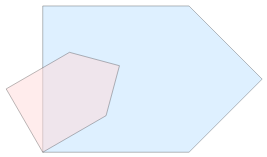
\includegraphics[scale=0.65]{./img/C4/ejemplo-ta-1.png} &   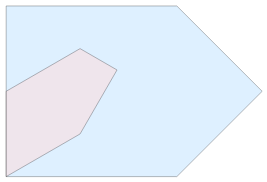
\includegraphics[scale=0.6]{./img/C4/ejemplo-ta-2.png} \\
    (a) $w=(0.5, 0.5, \frac{\pi}{6}, \frac{\pi}{6}, 0,0)$ & (b) $(0.5, 0.5, \frac{\pi}{6}, 0,0,0)$ \\[6pt]
    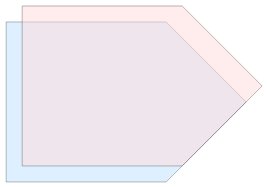
\includegraphics[scale=0.6]{./img/C4/ejemplo-ta-3.png} &   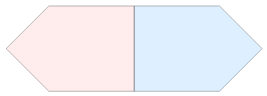
\includegraphics[scale=0.75]{./img/C4/ejemplo-ta-4.png} \\
    (c) $(1,1,0,0,0.1,0.1)$ & (d) $(1,1,\pi,0,0,0)$ \\[6pt]
    \end{tabular}
    \caption{Ejemplos de aplicaciones de transformaciones lineales}
    \label{fig:ejemplos-ta}
  \end{figure}

En el caso de (a) observamos una similitud con $r=0.5$ y $\alpha=\frac{\pi}{6}$. En (b) además de un escalado uniforme de razón $r=s=0.5$ podemos ver el efecto que tiene una rotación (no uniforme) en $X$ de razón $\alpha=\frac{\pi}{6}$. Por su parte, (c) simplemente aplica una traslación mediante el vector $b=(0.1,0.1)^t$. Por último, en (d) vemos un caso de reflexión respecto al eje $Y$.

Un último detalle para la creación de SFI es la necesidad de que las transformaciones afines utilizadas sean \textit{aplicaciones contractivas}. Procedemos por tanto a definir un SFI:

\begin{definicion}[Sistema de Funciones Iteradas]
    \label{def:SFI}
    Un \textbf{Sistema de Funciones Iteradas} se compone de un espacio métrico completo $(X,d)$ y de un conjunto finito de aplicaciones contractivas $w=\{w_i:i=1,\dots,n\}$.

    Se denomina \textit{constante de contractividad} del SFI a la mayor de las constantes de contractividad de las aplicaciones que lo forman, $s=\max\{s_i:i=1,\dots,n\}$, siendo $s_i$ la constante de contractividad de $w_i \ \ \forall i=1,\dots,n$.

    Dado un subconjunto $A\subseteq X$, la imagen de $A$ por medio de $w$ es definida como
    $$
    w(A)=\bigcup_{i=1}^n w_i(A).
    $$
\end{definicion}

Podemos utilizar como espacio métrico completo el plano euclídeo $\R^2$ y un conjunto finito de transformaciones lineales contractivas.

\begin{ejemplo}
    \label{ejemplo:sfi}
    Supongamos que tenemos un triángulo equilátero $T$ cuyos vértices son los puntos $(0,0),(1,0),(\frac{1}{2},\frac{\sqrt{3}}{2})$ y las transformaciones lineales
    \begin{eqnarray*}
        w_1 = \left(0.5,0.5,0,0,0,0\right) \\
        w_2 = \left(0.5,0.5,0,0,\frac 1 2,0\right) \\
        w_3 = \left(0.5,0.5,0,0,\frac 1 4,\frac{\sqrt{3}}{4}\right)
    \end{eqnarray*}
    Entonces en la imagen \ref{fig:ejemplo-sfi} podemos ver tanto $T$ como el resultado de aplicar el SFI $w=\{w_1,w_2,w_3\}$ a $T$.
    \begin{figure} [ht]
    \centering
    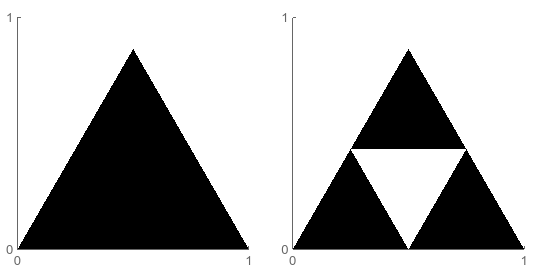
\includegraphics[scale = 0.6]{img/C4/ejemplo-sfi.png}
    \caption{Representación gráfica de $T$ y $w(T)$}
        \label{fig:ejemplo-sfi}
    \end{figure}
\end{ejemplo}

\section{Convergencia de SFI}
\label{section:convergencia-sfi}

Probablemente el resultado de aplicar el SFI $w$ a un triángulo equilátero que vemos en el ejemplo \ref{ejemplo:sfi} le recuerde al primer paso al generar el triángulo de Sierpinski, el cual vimos en la sección \ref{subsection:triangulo-Sierpinski}. De hecho, podemos volver a aplicar $w$ a $w(T)$, a $w(w(T))$, y así sucesivamente, de forma que iterando infinitamente $w$ en $T$, el resultado final que obtenemos es efectivamente el triángulo de Sierpinski \textbf{S}, véase de nuevo la imagen \ref{fig:triangulo-Sierpinski}.

Este es sólo un ejemplo, pero a lo largo de esta sección veremos que todo SFI converge a una figura, que denominamos el atractor del sistema, independientemente de la figura inicial. Véase en la figura \ref{fig:semillas-sfi} cómo incluso tomando como semilla una figura totalmente distinta al triángulo equilátero el resultado de la iteración es el mismo. Esto es de hecho una consecuencia del Teorema del punto fijo de Banach (teorema \ref{th:punto-fijo}).

\begin{figure} [ht]
    \centering
    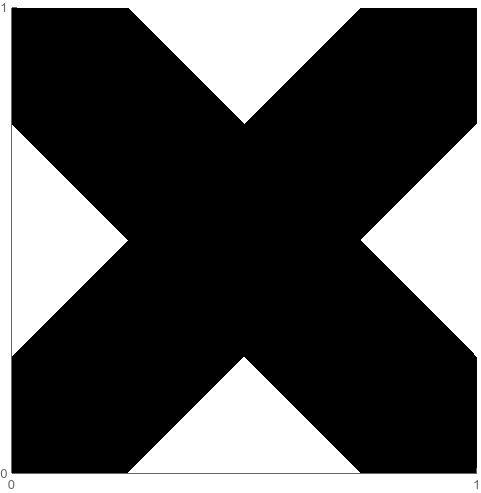
\includegraphics[scale = 0.33]{img/C4/figura-X.png}
    \caption{Otra posible semilla para iterar el SFI}
        \label{fig:semilla-X}
\end{figure}

\begin{figure}[ht]
    \centering
    \begin{tabular}{cc}
      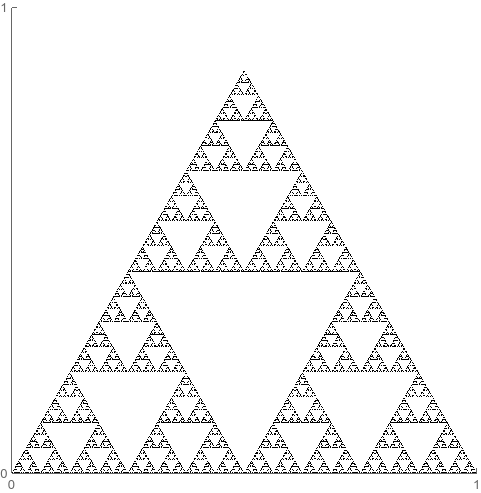
\includegraphics[scale=0.33]{./img/C4/triangulo-iterado.png} &   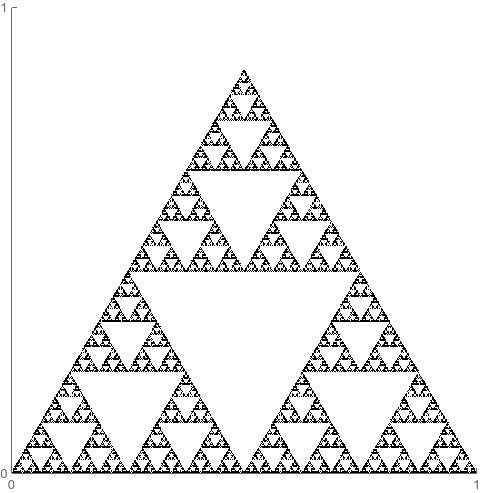
\includegraphics[scale=0.33]{./img/C4/figura-X-iterada.png} \\
    (a) Iterando un triángulo equilátero & (b) Iterando la figura \ref{fig:semilla-X} 
    \end{tabular}
    \caption{Resultado de iterar 8 veces $w$ con distintas figuras iniciales}
    \label{fig:semillas-sfi}
\end{figure}

\subsection{El Espacio de Fractales y la Métrica de Hausdorff}

Consideramos un espacio métrico completo $(X,d)$ y sea $\mathcal{H}(X)\subset\mathcal P (X)$ el conjunto de todos los subconjuntos compactos de $X$, el cual también se denomina \textit{espacio de fractales} de $X$. El objetivo ahora es dotar a $\mathcal{H}(X)$ de una distancia, la cual nos permita cuantificar la similaridad entre conjuntos compactos. 

Dado un punto $x\in X$ y un subconjunto $A\in\mathcal H(X)$ la distancia de un punto a un conjunto es definida como
$$
d(x,A) := \inf\{d(x,a):a\in A\}=\min\{d(x,a):a\in A\},
$$
donde el ínfimo es un mínimo porque $A$ es compacto. Si tomamos dos compactos $A,B\in\mathcal H(X)$, entonces la distancia de $A$ a $B$ se define como:
$$
d(A,B)=\max\{d(a,B):a\in A\}
$$

El problema es que esta definición no nos basta para definir una distancia entre conjuntos, pues si $A\subset B$ tenemos que $d(A,B)=0$, pero si $b\in B\backslash A$, entonces $d(b,A)>0$, por lo que necesariamente $d(B,A)>0$. Y como sabemos, una auténtica distancia es conmutativa. Véase el contraejemplo de la figura \ref{fig:contraejemplo-distancia}. 
\begin{figure} [ht]
    \centering
    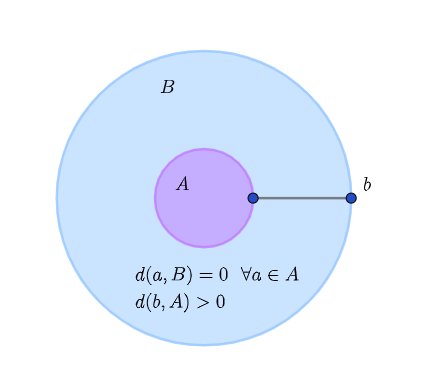
\includegraphics[scale = 0.4]{img/C4/no-distancia-hausdorff.png}
    \caption{Contraejemplo a la distancia entre conjuntos}
        \label{fig:contraejemplo-distancia}
\end{figure}

Por suerte, a partir de estas definiciones no es difícil encontrar una definición que cumpla las propiedades de una distancia.

\begin{definicion}
    Dado un espacio métrico completo $(X,d)$, en el espacio de fractales $\mathcal{H}(X)$ Se define la \textbf{distancia de Hausdorff} o \textbf{métrica de Hausdorff} como:
    $$
    h(d)(A,B)=\max\{d(A,B),d(B,A)\} \ \ \forall A,B\in\mathcal H(X).
    $$
\end{definicion}

En adelante denotaremos únicamente $h(\cdot,\cdot)$, omitiendo la dependencia de la distancia del espacio original.

Podemos comprobar en \cite[Sección 2.6]{Barnsley} que, en efecto, $h$ es una distancia. Además, en \cite[Sección 2.7]{Barnsley} se prueba que el espacio métrico $(\mathcal{H}(X), h(d))$ es completo.

\subsection{Aplicaciones contractivas en el espacio de fractales}

Consideramos un espacio métrico completo $(X,d)$ y su espacio de fractales dotado de la métrica de Hausdorff $(\mathcal H(X), h(d))$, que también es completo, y tomamos una aplicación contractiva $w:X\longrightarrow X$. Buscamos averiguar qué ocurre al iterar $w$ sobre $\mathcal{H}(X)$, siendo esta contractiva sobre $X$ y $\mathcal{H}(X)$ un espacio métrico completo. 

\begin{lema}
    \label{lema:contractivas-compactos}
    Sea $(X,d)$ un espacio métrico y $w:X\longrightarrow X$ una aplicación contractiva, entonces 
    $$w(\mathcal{H}(X))=\{w(A):A\in\mathcal{H}(X)\}\subseteq\mathcal{H}(X),$$
    es decir, la imagen por $w$ de todo compacto de $X$ es un conjunto compacto de $X$.
\end{lema}
\begin{proof}
    Sabemos que $w$ es continua en $X$, pues toda aplicación contractiva es lipschitziana y por tanto continua. Como la imagen de un conjunto compacto por una aplicación continua es un conjunto compacto, podemos afirmar que $w$ lleva elementos de $\mathcal{H}(X)$ a elementos de $\mathcal{H}(X)$.
\end{proof}

Ahora necesitamos alguna forma de construir aplicaciones contractivas en el espacio $(\mathcal{H}(X),h)$ a partir de aplicaciones contractivas en $(X,d)$. Gracias al siguiente lema comprobamos que la forma más natural es suficiente.

\begin{lema}
    Sea $(X,d)$ un espacio métrico y $w:X\longrightarrow X$ una aplicación contractiva con constante de Lipschitz $s$. Entonces $w:\mathcal{H}(X)\longrightarrow\mathcal{H}(X)$, definida naturalmente como
    $$
    w(A)=\{w(a):a\in A\}\ \ \forall A\in\mathcal{H}(X)
    $$
    es una aplicación contractiva en $(\mathcal{H}(X),h)$.
\end{lema}
\begin{proof}
    Si utilizamos el lema \ref{lema:contractivas-compactos} podemos afirmar que la aplicación $w:\mathcal{H}(X)\longrightarrow\mathcal{H}(X)$ está bien definida, por lo que falta probar que en efecto es contractiva. Sean $A,B\in\mathcal{H}(X)$, tenemos que
    \begin{eqnarray*}
        d(w(A),w(B)) & = & \max\left\lbrace \min \left\lbrace d(w(a),w(b)): b\in B\right\rbrace : a\in A \right\rbrace \\
                     & \leq &  \max\left\lbrace \min \left\lbrace s\cdot d(a,b): b\in B\right\rbrace : a\in A \right\rbrace \\
                     & = & s\cdot d(A,B).
    \end{eqnarray*}
    Análogamente, $d(w(B),w(A))\leq s\cdot d(B,A)$. Por tanto
    \begin{eqnarray*}
        h(w(A),w(B)) & = & \max \{d(w(A),w(B)), d(w(B),w(A))\} \\
                     & \leq & s \max \{d(A,B), d(B,A))\} \\
                     & = & s\cdot h(A,B).
    \end{eqnarray*}
    Por lo que tenemos que $w$ es contractiva sobre $\mathcal{H}(X)$.
\end{proof}

Enunciamos una propiedad de la métrica de Hausdorff $h$ que nos hará falta dentro de poco.

\begin{lema}
    \label{lema:uniones}
    Sean $A,B,C,D\in\mathcal{H}(X)$, entonces 
    $$h(A\cup B, C\cup D)\leq\max\{h(A,C),h(B,D)\}.$$
\end{lema}
\begin{proof}
    La prueba se sigue de otra propiedad de la distancia $d$:
    \begin{eqnarray*}
    d(A\cup B,C) & = & \max\{d(x,C)\ \ \forall x\in A\cup B\} \\
                 & = & \max\left\lbrace \max\left\lbrace d(x,C):x\in A \right\rbrace, \max\left\lbrace d(x,C):x\in B \right\rbrace\right\rbrace \\
                 & = & \max\left\lbrace d(A,C),d(A,B) \right\rbrace.
    \end{eqnarray*}
    Y de esta igualdad se deduce la desigualdad pedida. %TODO aunque no se muy bien como.
\end{proof}

Seguidamente presentamos un resultado que nos ayuda a construir aplicaciones contractivas en $\mathcal{H}(X)$ a partir de no sólo una sino de varias aplicaciones contractivas en $X$, a través del cual enlazaremos, esta vez en un contexto más teórico y formal, con la definición de SFI como conjunto de aplicaciones contractivas en un espacio métrico completo.

\begin{proposicion}
    Sea $(X,d)$ un espacio métrico y sea $\{w_i:i=1,\dots,n\}$ un conjunto finito de aplicaciones contractivas $w_i:\mathcal{H}(X)\longrightarrow\mathcal{H}(X)$, cada una con constante de contractividad $s_i$. Definimos la aplicación $W:\mathcal{H}(X)\longrightarrow\mathcal{H}(X)$ como
    \begin{equation}
        \label{eqn:W}
        W(A) := \bigcup_{i=1}^n w_i(A) \ \ \forall A\in\mathcal{H}(X).
    \end{equation}
    Entonces $W$ es una aplicación contractiva en $\mathcal{H}(X)$ y su constante de contractividad es $s=\max\{s_i:i=1,\dots,n\}$.
\end{proposicion}
\begin{proof}
    Demostraremos el caso $n=2$, de forma que por inducción sería cierto para cualquier $n\leq 1$. Sean $A,B\in\mathcal{H}(X)$, tenemos que
    \begin{eqnarray*}
    h(W(A),W(B)) & = & h(w_1(A)\cup w_2(A), w_1(B)\cup w_2(B)) \\
                 & \leq & \max\{h(w_1(A),w_1(B)), h(w_2(A),w_2(B))\}\text{ (lema \ref{lema:uniones})} \\
                 & \leq & \max\{s_1\cdot h(A,B), s_2\cdot h(A,B) \} \\
                 & \leq & \max\{s_1,s_2\} h(A,B) \\
                 & = & s \cdot h(A,B)
    \end{eqnarray*}
    Lo cual completa la demostración.
\end{proof}

\subsection{El espacio de fractales y los SFI}

Hasta ahora hemos probado varios resultados que nos han servido para construir aplicaciones contractivas en el espacio de fractales de un espacio métrico a partir de un conjunto finito de aplicaciones contractivas. Si añadimos la hipótesis de la complitud, tendríamos con ese conjunto de aplicaciones contractivas un SFI, el cual podemos iterar bajo la seguridad de que no perdemos dicha contractividad. Por lo tanto, y recuperando la definición \ref{def:SFI}, ya podemos recopilar toda la información que tenemos y enunciar el siguiente teorema:

\begin{teorema}
    Consideramos el SFI formado por el espacio métrico completo $(X,d)$ y el conjunto $\{w_i:i=1\dots, N\}$ de aplicaciones contractivas, siendo $s$ la constante de contractividad del SFI. Consideramos también el espacio de fractales $(\mathcal{H}(X),h)$, donde definimos la aplicación $W:\mathcal{H}(X)\longrightarrow\mathcal{H}(X)$ como en (\ref{eqn:W}):
    $$
    W(A) := \bigcup_{i=1}^N w_i(A) \ \ \forall A\in\mathcal{H}(X).
    $$
    Entonces $W$ es una aplicación contractiva de constante $s$ y admite un único punto fijo $A^*\in\mathcal{H}(X)$, el cual está dado por 
    $$
    A^*=\lim_{n\rightarrow\infty} W^n(B) \ \ \forall B\in\mathcal{H}(X).
    $$

\end{teorema}
\begin{proof}
    Gracias a los resultados anteriores solo nos quedaría probar que $W$ admite un único punto fijo dado por la iteración infinita de $W$ e independientemente de qué $B\in\mathcal{H}(X)$ inicial se tome. Sin embargo, teniendo en cuenta que $W$ es contractiva y que $\mathcal{H}(X)$ es un espacio métrico completo, simplemente aplicando el teorema del punto fijo de Banach (teorema \ref{th:punto-fijo}) se tiene el resultado completo
\end{proof}

En resumen, tenemos que todo SFI admite un único punto fijo al que converge la iteración sucesiva de la aplicación $W$ construida a partir de su conjunto de aplicaciones contractivas. Además, esta convergencia está asegurada sea cual sea el conjunto inicial en el que se comienzan las iteradas. Como veníamos anunciando al inicio de esta sección, podemos ponerle nombre al punto fijo del SFI:

\begin{definicion}[Atractor]
    Dado un SFI, definimos que su único punto fijo como el \textbf{atractor} del SFI.    
\end{definicion}

Recordamos ahora el SFI del ejemplo \ref{ejemplo:sfi} y las imágenes \ref{fig:semillas-sfi}, que nos permitirían comprobar que el triángulo de Sierpinski es el atractor del SFI y que independientemente de la figura inicial (siempre y cuando sea un conjunto compacto de $\R^2$) la iteración conjunta de $\{w_1,w_2,w_3\}$ converge a $\mathbf{S}$ como resultado.

Ahora podemos aplicar esta teoría al espacio métrico completo $\R^2$ y a las transformaciones afines, que para asegurar la convergencia necesitamos que sean contracciones. Afortunadamente, es sencillo probar esta condición.

\begin{proposicion}
    Sea $w =(r,s,\alpha,\beta,e,f)$ una transformación afín de $\R^2$. Si $\alpha=\beta$ y $\max\{|r|,|s|\}\leq 1$, entonces $w$ es una aplicación contractiva. 
\end{proposicion}
\begin{proof}
    Por un lado, las rotaciones uniformes y las traslaciones son movimientos rígidos, en particular aplicaciones lipschitzianas de constante de Lipschitz igual a 1. Por tanto, por composición, para comprobar que $w$ es contractiva, debemos probar que un escalado (uniforme o no) es una aplicación contractiva si $\max\{|r|,|s|\}<1$. Supongamos que la aplicación $s(x_1,x_2)=(r\cdot x_1,s\cdot x_2)$ verifica $K=\max\{|r|,|s|\}\leq 1$. Entonces, para cualesquiera $x=(x_1,x_2), y=(y_1,y_2)\in\R^2$:
    \begin{eqnarray*}
        \|s(x) - s(y)\| & = & \|(s_1 x_1-s_1 y_1, s_2 x_2 - s_2 y_2)\| \\
                        & = & \|(s_1(x_1-y_1), s_2(x_2-y_2))\| \\
                        & \leq & K \|x-y\|
    \end{eqnarray*}
    Por tanto $s$ es contractiva.
\end{proof}

Y una vez que sabemos cómo hacer que una transformación afín sea contractiva, podemos , sin importar el conjunto de partida, obtener imágenes fractales a partir únicamente de una colección finita de sextuplas, cada una representando una transformación afín contractiva. Como posibles ejemplos, y para que se observe la diversidad que ofrece este método, en las tablas \ref{tabla:arbol-pitagoras} y \ref{tabla:helecho-Barnsley} se pueden observar los SFI cuyos atractores son el árbol pitagórico y el helecho de Barnsley (imágenes \ref{fig:atractores-sfi} (a) y (b) respectivamente), siendo este último una imagen cuya representación es ya bastante realista.

\newpage
\begin{table}
    \centering
    \begin{tabular}{c|cccccc} \hline
        $w$ & $r$ & $s$ & $\alpha$ & $\beta$ & $e$ & $f$ \\ \hline\hline
    1 & 1 & 1 & 0 & 0 & 0 & 0 \\ \hline
    2 & $1/\sqrt 2$ & $1/\sqrt 2$ & $\pi/4$ & $\pi/4$ & 0 & 1 \\ \hline
    3 & $1/\sqrt 2$ & $1/\sqrt 2$ & $-\pi/4$ & $-\pi/4$ & $1/2$ &  $3/2$ \\ \hline
    \end{tabular}
    \caption{SFI para el árbol pitagórico}
    \label{tabla:arbol-pitagoras}
\end{table}

\begin{table}
    \centering
    \begin{tabular}{c|cccccc} \hline
        $w$ & $r$ & $s$ & $\alpha$ & $\beta$ & $e$ & $f$ \\ \hline\hline
    1 & 0.85 & 0.85 & $-\pi/72$ & $-\pi/72$ & 0 & 1.6 \\ \hline
    2 & 0.3 & 0.34 & $49 \pi/180$ & $49 \pi/180$ & 0 & 1.6 \\ \hline
    3 & 0.3 & 0.34 & $2 \pi/3$ & $2 \pi/3$ & 0 & 0.44 \\ \hline
    4 & 0 & 0.3 & 0 & 0 & 0 & 0 \\ \hline
    \end{tabular}
    \caption{SFI para el helecho de Barnsley}
    \label{tabla:helecho-Barnsley}
\end{table}

\begin{figure}[ht]
    \centering
    \begin{tabular}{cc}
      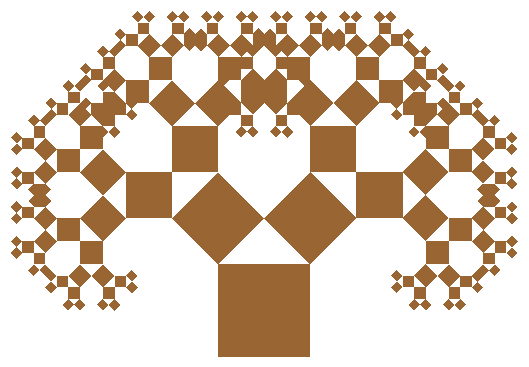
\includegraphics[scale=0.5]{./img/C4/arbol-pitagoras.png} &   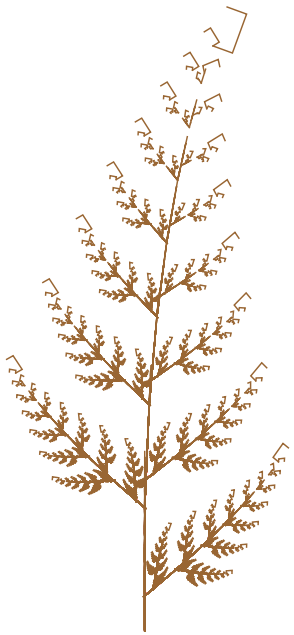
\includegraphics[scale=0.4]{./img/C4/helecho-barnsley.png} \\
    (a) Árbol pitagórico & (b) Helecho de Barnsley 
    \end{tabular}
    \caption{Atractores de los SFI definidos en las tablas \ref{tabla:arbol-pitagoras} y \ref{tabla:helecho-Barnsley}.}
    \label{fig:atractores-sfi}
\end{figure}

\section{SFI y conjuntos autosimilares}
\label{section:sfi-conjuntos-autosimilares}

En el capítulo \ref{chap:concepto} y concretamente en la sección \ref{subsection:relacion-dimensiones} presentamos algunas relaciones entre los distintos tipos de dimensión, y en la sección \ref{subsection:dim-cajas} hablamos de la dimensión por cajas de un conjunto. Si nos restringimos a conjuntos autosimilares el cálculo de la dimensión por cajas se simplifica gracias a algunos resultados que le debemos a la teoría de los SFI. Para ello, previamente introducimos la siguiente definición.

\begin{definicion}
    \label{def:condicion-conjunto-abierto}
    Sean $(X,d)$ un espacio métrico completo y un SFI $w=\{w_i:i=1,\dots,n\}$ en $X$. $w$ satisface la \textbf{condición de conjunto abierto} si existe un conjunto abierto $\emptyset\not= U\subseteq X$ tal que las imágenes $w_1(U),\dots,w_n(U)\subseteq U$ y son disjuntas.
\end{definicion}

Intuitivamente, esta condición nos afirma que podemos controlar el `tamaño' del resultado de aplicar el SFI y que además las imágenes de cada aplicación que compone el SFI no se solapan unas con otras. Gracias a esta condición podemos enunciar el siguiente teorema, que es el que nos proporcionará las herramientas esenciales para el cálculo de la dimensión en estos casos.

\begin{teorema}
    \label{th:Moran}
    Sean $(X,d)$ un espacio métrico completo, un SFI $w=\{w_i:i=1,\dots,n\}$ en $X$ que satisface la condición de conjunto abierto y $\{c_i:i=1,\dots,n\}$ las constantes de contractividad de las aplicaciones $w_i$. Entonces la dimensión por cajas del atractor de $w$ es el único valor real positivo $d$ que satisface la ecuación $1 = c_1^d + \cdots c_n^d$ y esta coincide con la dimensión de Hausdorff.
\end{teorema}

Podemos encontrar la prueba de este teorema en \cite{Moran}.

\begin{corolario}
    En caso de que todas las constantes de contractividad sean iguales a cierta constante $0<c<1$, entonces la dimensión $d$ es
    $$
    d = \dfrac{\log(n)}{\log(1/c)}.
    $$
\end{corolario}

\begin{observacion}
    En $\R^2$, a partir de un conjunto autosimilar según la definición \ref{def:autosimilaridad} podemos construir un SFI cuyo atractor sea el propio conjunto autosimilar.
\end{observacion}

Mediante el teorema de Moran y viendo ciertos fractales como atractores de SFI podemos rápidamente calcular su dimensión por cajas. Por ejemplo, el triángulo de Sierpinski es el atractor del SFI presentado en el ejemplo \ref{ejemplo:sfi}. El SFI cumple la condición de conjunto abierto tomando como $U$ el interior del propio triángulo equilátero inicial y viendo, como podemos observar en la imagen \ref{fig:ejemplo-sfi} que las imágenes por cada una de las aplicaciones no salen del triángulo y además son disjuntas.  En este caso tenemos tres similitudes, en todas ellas la constante de contractividad es $\frac{1}{2}$, por lo que aplicando el corolario su dimensión por cajas es $\dim_B(\mathbf{S})=\frac{\log(3)}{\log(2)}$, como ya calculamos en la sección \ref{subsection:dim-cajas}.

Es por tanto el momento de calcular la dimensión por cajas de la curva de Koch \textbf{K}, la cual no hemos calculado aún. La curva de Koch es el atractor del SFI definido por las transformaciones especificadas en la tabla \ref{tabla:curva-koch}. Fijémonos que son $4$ transformaciones afines, todas ellas similitudes cuya homotecia tiene la misma razón: $\frac{1}{3}$. Por tanto, aplicando el corolario, vemos que
$$
\dim_B(\mathbf{K})=\dfrac{\log(4)}{\log(3)} \approx 1.2618,
$$
que es un valor situado entre 1 y 2.

\begin{table}[ht]
    \centering
    \begin{tabular}{c|cccccc} \hline
        $w$ & $r$ & $s$ & $\alpha$ & $\beta$ & $e$ & $f$ \\ \hline\hline
    1 & $1/3$ & $1/3$ & 0 & 0 & 0 & 0 \\ \hline
    2 & $1/3$ & $1/3$ & $\pi/3$ & $\pi/3$ & $1/3$ & 0 \\ \hline
    3 & $1/3$ & $1/3$ & $-\pi/3$ & $-\pi/3$ & $1/2$ & $\sqrt{3}/6$ \\ \hline
    4 & $1/3$ & $1/3$ & 0 & 0 & $2/3$ & 0 \\ \hline
    \end{tabular}
    \caption{SFI para la curva de Koch}
    \label{tabla:curva-koch}
\end{table}



\section{El problema inverso}

Como ya hemos podido ver, los SFI nos abren un mundo de posibilidades para crear imágenes fractales, ya que todos convergen a un atractor. Sin embargo, podemos también plantearnos el problema inverso. A partir de una imagen, ¿es posible determinar un SFI tal que su atractor sea la imagen inicial? Este es el punto clave de la teoría de la compresión por imágenes fractales. Pensemos que es mucho más ligero almacenar en memoria un conjunto finito de números en coma flotante que una imagen (viéndose esta como una colección de píxeles).

En este contexto, la mejor herramienta que tenemos es el conocido como \textit{teorema del collage}, que enunciamos a continuación.

\begin{teorema}[El teorema del collage]
    Sean $(X,d)$ un espacio métrico completo, $L\in\mathcal{H}(X)$ y $\varepsilon\geq 0$. Si $\{w_i:i=1,\dots,N\}$ es un SFI en $X$ con constante de contractividad $0\leq s < 1$ cumpliendo que
    $$
    h\left(L,\bigcup_{i=1}^N w_i(L)\right) \leq \varepsilon,
    $$
    donde $h(d)$ es la métrica de Hausdorff, entonces
    $$
    h(L,A)\leq \dfrac{\varepsilon}{1-s}
    $$
    donde $A$ es el atractor del SFI. Equivalentemente,
    $$
    h(L,A)\leq(1-s)^{-1} h\left(L, \bigcup_{i=1}^N w_i(L)\right) \ \ \forall L\in\mathcal{H}(X).
    $$
\end{teorema}

Para probar el teorema del collage primero probamos el siguiente lema, que nos deja la mayor parte del trabajo hecho.

\begin{lema}
    Sea $(X,d)$ un espacio métrico completo. Sea $f:X\longrightarrow X$ una aplicación contractiva con constante de contractividad $0\leq s < 1$ y consideramos $x^*\in X$ el punto fijo de $f$. Entonces
    $$
    d(x,x^*)\leq (1-s)^{-1} d(x,f(x)) \ \ \forall x\in X.
    $$
    \label{lema:collage}
\end{lema}
\begin{proof}
    Fijado $x\in X$, la función distancia $d(x,\cdot)$ es continua, por tanto:
    \begin{eqnarray*}
        d(x,x^*) & = & d(x,\lim_{n\rightarrow\infty} f^n(x)) = \lim_{n\rightarrow\infty} d(x,f^n(x)) \\
        & \leq & \lim_{n\rightarrow\infty} \sum_{i=1}^n d(f^{i-1}(x),f^{i}(x)) \ \ \text{(desigualdad triangular)}\\ 
        & \leq & \lim_{n\rightarrow\infty} d(x,f(x))\sum_{i=1}^n s^{i-1} \\
        & = & (1-s)^{-1} d(x,f(x))
    \end{eqnarray*}
    donde en la última igualdad hemos utilizado que la suma de los elementos de una serie geométrica de razón $0\leq\alpha<1$ es $(1-\alpha)^{-1}$.
\end{proof}

Aplicando el lema \ref{lema:collage} al espacio métrico $(\mathcal{H}(X), h(d))$ y a la aplicación contractiva $W$ generada por $\{w_i:i=1,\dots,N\}$ como en (\ref{eqn:W}) tenemos probado el teorema del collage.

Intuitivamente, este teorema nos dice que para encontrar un SFI cuyo atractor es similar a un conjunto dado, debemos buscar un conjunto finito de aplicaciones contractivas (transformaciones afines contractivas en $\R^2$) tales que la unión (el collage) formada por las imágenes del conjunto dado vía dichas aplicaciones se parezca a sí mismo. La forma de medir esta similaridad de manera cuantitativa es mediante la métrica de Hausdorff.

\begin{ejemplo}
    Vamos a aplicar el teorema del collage para encontrar un SFI que nos ayude a replicar la imagen \ref{fig:ejemplo-collage} (a).
    \begin{figure}[ht]
        \centering
        \begin{tabular}{cc}
          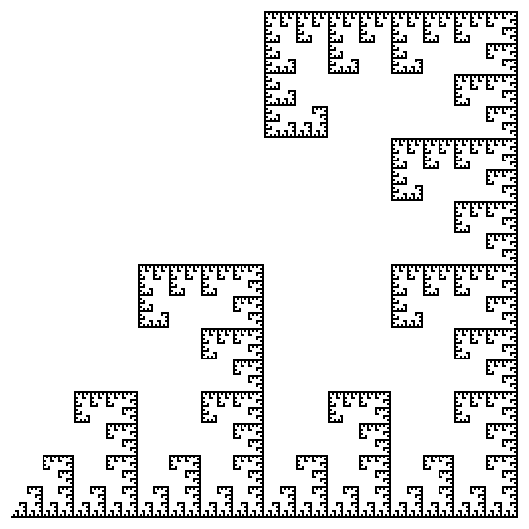
\includegraphics[scale=0.45]{./img/C4/ejemplo-collage-original.png} &   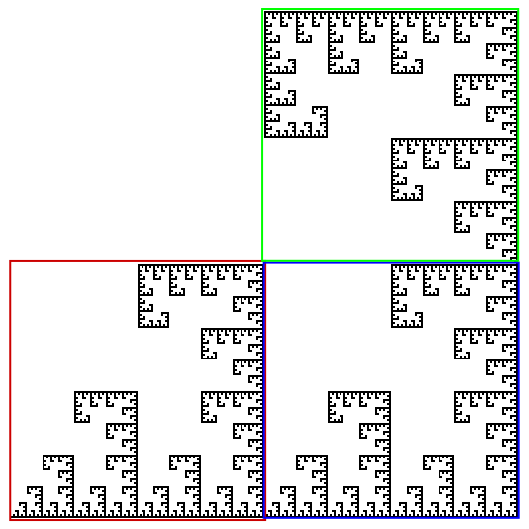
\includegraphics[scale=0.34]{./img/C4/ejemplo-collage.png} \\ (a) & (b) \\
        \end{tabular}
        \caption{Imagen cuyo SFI debemos determinar}
        \label{fig:ejemplo-collage}
    \end{figure}

    Para ello, siguiendo lo que nos sugiere el teorema del collage debemos encontrar transformaciones afines tales que la unión de las imágenes de este conjunto sea lo más parecida posible al conjunto original. Llamemos $L$ al subconjunto de $\R^2$ que representa este fractal.

    Fijémonos, tal y como se puede ver en la imagen \ref{fig:ejemplo-collage} (b) que $L$ está compuesto por tres copias reducidas de sí mismo. Por lo que trataremos de buscar tres transformaciones afines tales que cada una genere una de las copias del propio $L$, de forma que al unirlas obtendríamos de nuevo el mismo conjunto.
    \begin{itemize}
        \item La copia \textcolor{red}{roja} es simplemente el propio $L$ contraído a la mitad en ambos ejes, por lo que utilizamos la aplicación $\textcolor{red}{w_1=(0.5,0.5,0,0,0,0)}$.
        \item La copia \textcolor{blue}{azul} es, al igual que la \textcolor{red}{roja}, el resultado de aplicar una homotecia de razón 0.5, pero esta vez también se desplaza 0.5 unidades a la derecha. La aplicación que buscamos es por tanto $\textcolor{blue}{w_2=(0.5,0.5,0,0,0.5,0)}$.
        \item Por último, la copia \textcolor{green}{verde} debemos fijarnos que además de escalada y desplazada, está girada. Por lo que es el resultado de aplicar una similitud de razón de homotecia $0.5$ y ángulo de rotación $\frac \pi 2$, para posteriormente colocar este resultado encima de la copia \textcolor{blue}{azul}. Es decir, usamos la transformación $\textcolor{green}{w_3=(0.5,0.5,\frac{\pi}{2},\frac{\pi}{2},1,0.5)}$.
    \end{itemize}

    Por tanto, $L$ es el atractor del siguiente SFI:

    \begin{table}[ht]
        \centering
        \begin{tabular}{c|cccccc} \hline
        $w$ & $r$ & $s$ & $\alpha$ & $\beta$ & $e$ & $f$ \\ \hline\hline
        1 & 0.5 & 0.5 & 0 & 0 & 0 & 0 \\ \hline
        2 & 0.5 & 0.5 & 0 & 0 & 0.5 & 0 \\ \hline
        3 & 0.5 & 0.5 & $\frac{\pi}{2}$ & $\frac{\pi}{2}$ & 1 &  0.5 \\ \hline
        \end{tabular}
        \caption{SFI para la imagen \ref{fig:ejemplo-collage}}
        \label{tabla:ejemplo-collage}
    \end{table}
\end{ejemplo}

Para una mayor cantidad y variedad de ejemplos invitamos al lector a consultar \cite[Sección 3.10]{Barnsley}, donde puede encontrar gran cantidad de ejercicios y explicaciones prácticas y más complejas.

En conclusión, los SFI en $\R^2$ a pesar de ser herramientas muy simples como lo son las transformaciones afines, nos permiten originar complejas y bellas imágenes basadas en la iteración. Además, gracias al teorema del collage podemos aproximar una imagen simplemente a partir de las transformaciones afines que definen un SFI que converge a dicha aproximación. Toda esta teoría está además basada en una densa teoría que gira en torno al teorema del punto fijo de Banach.

